\chapter{ATLAS トリガーシステム}\label{chapter3}

\section{ATLASトリガーシステムの概要}\label{chapter3-1}
ATLAS実験では陽子陽子衝突が40MHzで起こるので、すべての事象に対して処理を行い、記録することは不可能である。
そのため、膨大な数のデータの中から興味のある事象のみを選別して保存している。このシステムは「トリガーシステム」と呼ばれる。
トリガーシステムは測定したい物理に対して様々な種類が用意されており、ミューオン、電子、光子、タウ、ジェットなどの種類がある。事象の選別では、横運動量やエネルギーに対して閾値を設けて、単位時間当たりに処理するイベントの数(トリガーレート)が使用できるデータ資源を超えないように行われる。

このトリガーシステムは、ATLAS実験では2段階で構成されている。ハードウェアを用いて高速演算を行う初段トリガー(Level-1 trigger)とソフトウェアを用いて精密処理を行う後段トリガー(High Level trigger)である。トリガーシステムによって、トリガーレートはL1で約100kHzまで落とされ、HLTで約1kHz程度まで削減され、記録される。

以下ではATLAS実験におけるミューオントリガーについて説明する。

\section{ミューオントリガーシステム}\label{chapter3-2}
図~\ref{fig:3-1}にミューオントリガー全体のデータの流れを示す。

\begin{figure}[h]
  \centering
  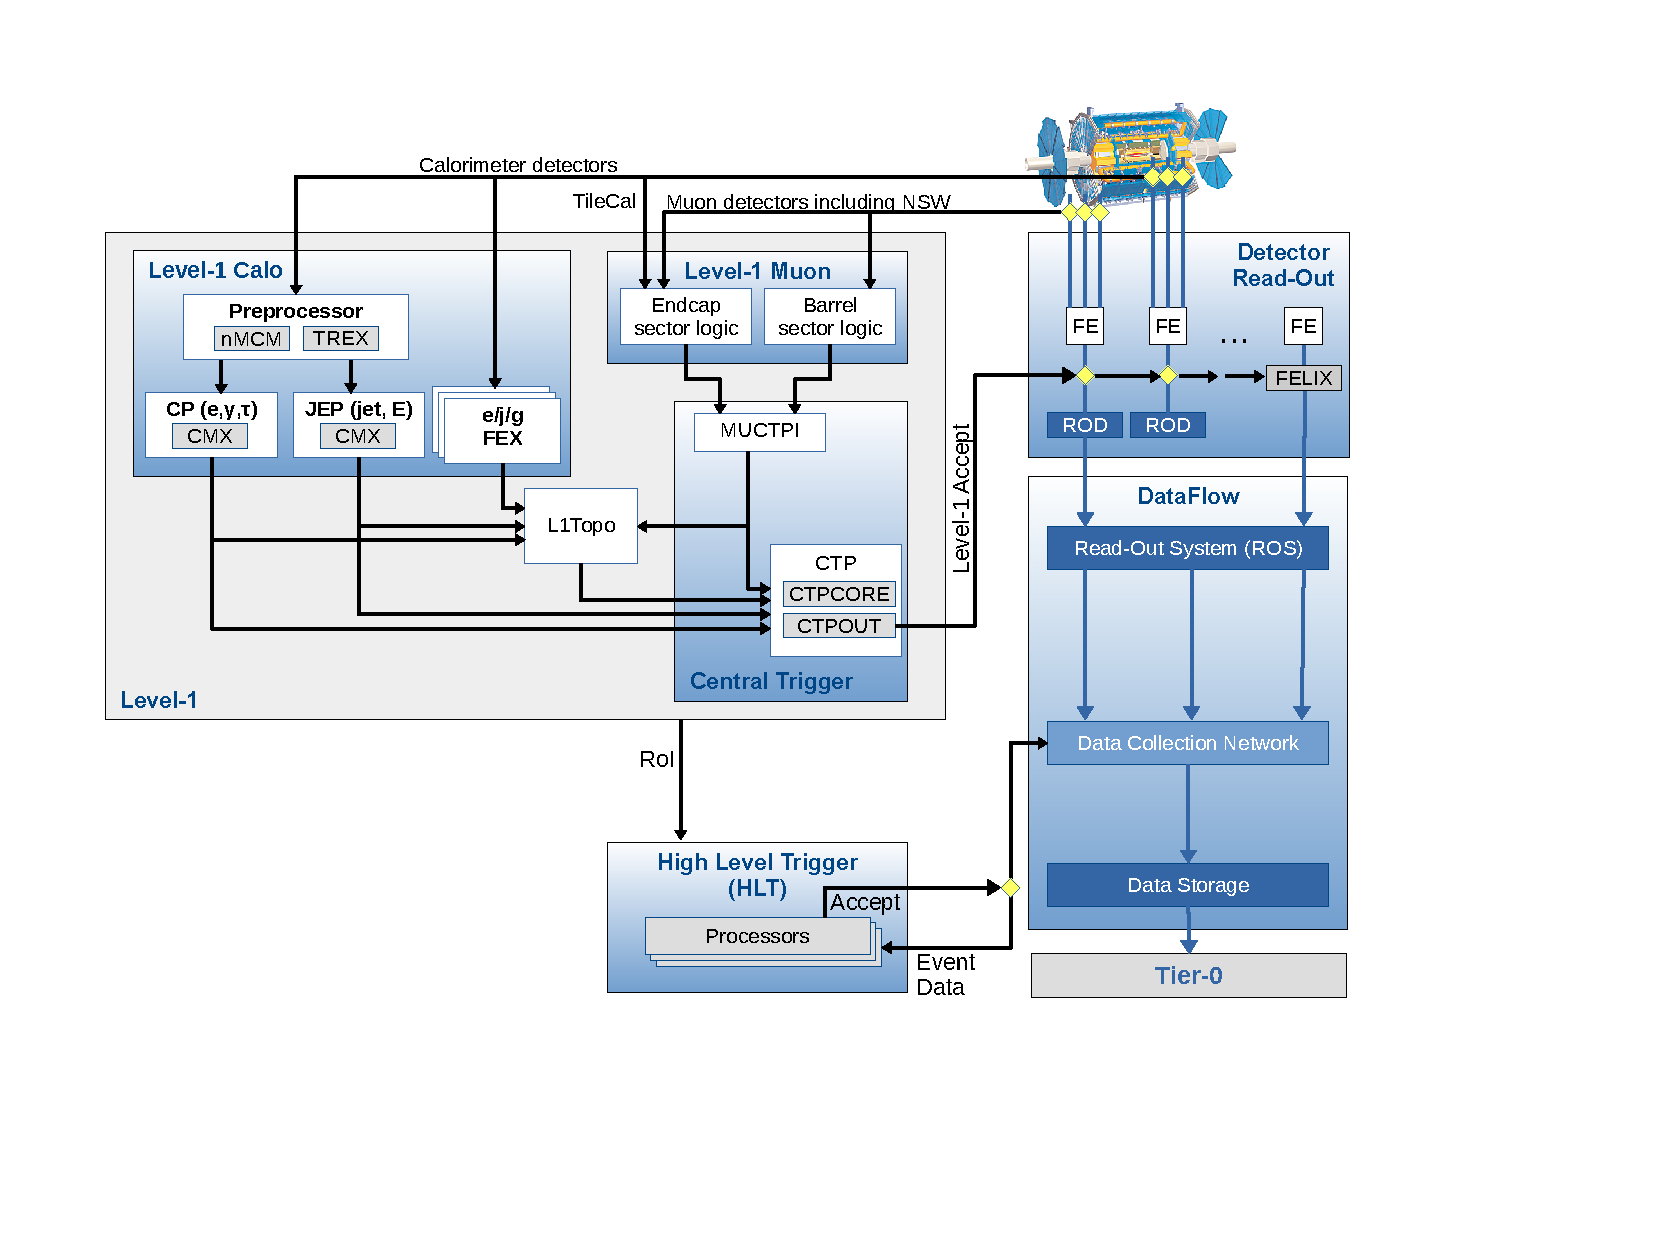
\includegraphics[clip, width=14cm]{fig/3/tdaq-run3-schematic.pdf}
  \caption{Run-3におけるミューオントリガーシステム全体のデータフロー\cite{article:approvedPlotsDAQ}。}
  \label{fig:3-1}
\end{figure}

L1でトリガー判定を行い判定をクリアしたミューオンに対して、大まかな通過位置を示す~Region~of~Interest~(RoI)を発行する。
HLTではL1から送られてきたRoIが持つ$\eta$、$\phi$の情報をもとに、RoI周辺の検出器の情報を用いて部分飛跡の再構成を行い、飛跡から求めた$p_T$に対して閾値を設けることでトリガー判定を行う。

HLTでは複数の段階で部分飛跡を再構成している。
まずRoI周辺のミューオン検出器の情報のみを用いてミューオンの部分飛跡を再構成する~Level-2~StandAlone~muon~trigger~(L2MuonSA)、次にL2MuonSAの情報と内部飛跡検出器の情報を組み合わせることによってより正確な飛跡の再構成と$p_T$の計算を行う~Level-2~Combined~muon~trigger~(L2MuonCB)、最後にここまでで選別されてきた事象に対しオフライン再構成と同等のアルゴリズムを用いることで、正確に$p_T$を計算し、トリガー判定を行う~Event~Filter~(EF)である。
以下でそれぞれの詳細について述べる。

\subsection{初段トリガーシステム~(Level-1 Trigger)}\label{chapter3-2-1}
ここでは、L1トリガーについて、バレル領域とエンドキャップ領域それぞれについて説明する。
図~\ref{fig:3-2}ではバレル領域、エンドキャップ領域それぞれでのL1ミューオントリガーアルゴリズムの概念図を示す。

\begin{figure}[h]
  \centering
  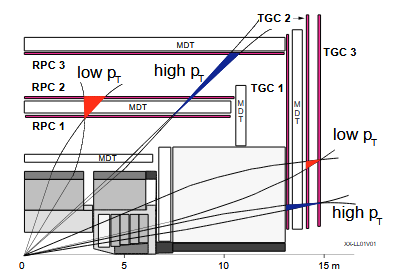
\includegraphics[clip, width=13cm]{fig/3/muon_trigger_overview.png}
  \caption{L1ミューオントリガーの概念図\cite{article:barrelSystem}。}
  \label{fig:3-2}
\end{figure}

\subsubsection{バレル領域}
バレル領域ではRPCのヒット情報を用いてミューオンの再構成を行う。2章で述べたようにRPCはミドルステーションに~RPC1と~RPC2の2層、アウターステーションに~RPC3の1層の合計3層が配置されている。RPCのそれぞれの層は、$\eta$、$\phi$方向の測定を行うために$\eta$stripと$\phi$stripを重ねたダブレット構造のストリップ層が2層で構成されている。
トリガーアルゴリズムは、以下の通りである。
まず~RPC2にヒットがあることを要求し、このヒットの点と衝突点を結ぶ直線を探索領域~(ロード)の中心として定義し、ロード内にある~RPC1のヒットを探索する。探索領域の幅は要求する$p_T$閾値によって決まる。$p_T$しきい値が高いときのみ~RPC3のヒットも用いる。
これはミューオンはトロイド磁石によって$\eta$方向に曲げられ、曲率は$p_T$に依存しているので、高い$p_T$を持つミューオンほど磁場で曲げられず衝突点から真っ直ぐ飛び~RPC3を通過しやすくなるからである。
低い$p_T$を持つミューオンのトリガー判定はRPC1とRPC2で行い、高い$p_T$を持つミューオンのトリガー判定は~RPC1と~RPC2、RPC3で行う。

この領域におけるL1トリガーは、$\eta$、$\phi$方向にそれぞれ32分割された合計64層のそれぞれ独立なトリガーセクターごとに判定が行われる。
さらに各セクターは$\Delta\eta\times\Delta\phi=0.2\times0.1$、$\Delta\eta\times\Delta\phi=0.1\times0.2$の大きさ~Coincidence~matrix($\eta$-CM、$\phi$-CM)に区分され、このCM単位で~RPC1と~RPC2または~RPC2と~PRC3のコインシデンスを取り、$p_T$の閾値の判定を行う。
隣接する2つずつの$\eta$-CM、$\phi$-CMはまとめて~Padと呼ばれる。このPadは$\eta\times\phi=0.2\times0.2$の大きさで、ミューオンの通過領域を表す~RoIが4つで構成される。RoIは$\eta$-CM、$\phi$-CMが重なる$\eta\times\phi=0.1\times0.1$の大きさの領域であり、Pad1つに付き最大1つしか定義できない。L1で定義した~RoIの情報は後段ミューオントリガーに送られる。$\eta$-CM、$\phi$-CM、Pad、RoIの概念図を図~\ref{fig:3-3}に示す。

\begin{figure}[h]
  \centering
  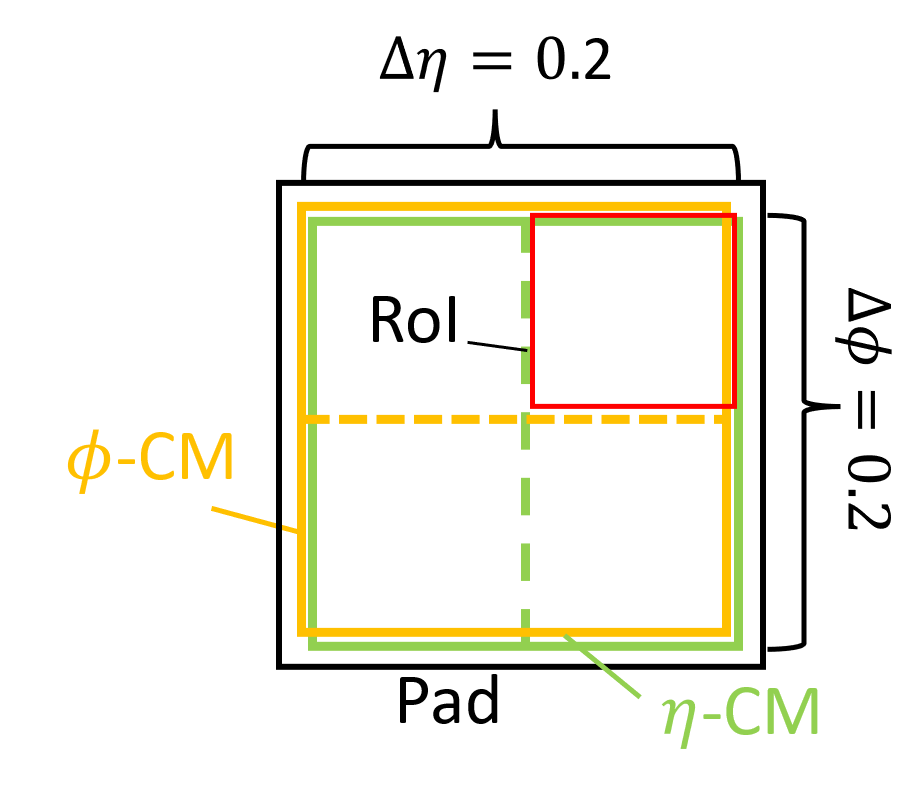
\includegraphics[clip, width=6cm]{fig/3/L1_CM.png}
  \caption{バレル領域における~Coincidence matrix~(CM)の概念図。}
  \label{fig:3-3}
\end{figure}

\subsubsection{エンドキャップ領域}
エンドキャップ領域では2章で示したTGCのヒット情報を用いてミューオンの再構成を行う。
TGCはインナーステーションに1枚~(I)、ミドルステーションに3枚~(M1、M2、M3)配置されている。
トリガーアルゴリズムは以下の通りである。
まずM3にヒットがあることを要求し、M3のヒットと衝突点を結ぶ直線のロードの中心として定義する。ミューオンは検出器より内側のトロイド磁場によって曲げられてTGCに入射するので、図~\ref{fig:3-4}のようにM1において実際のヒット点と直線は~dR、d$\phi$だけずれる。
あらかじめ作成されている~dR、d$\phi$と$p_T$の対応関係を示した~Coincidence~Window~(CW)図~\ref{fig:3-5}を用いて、~dR、d$\phi$から$p_T$を計算することで短時間での$p_T$判定を行っている。

\begin{figure}[h]
  \centering
  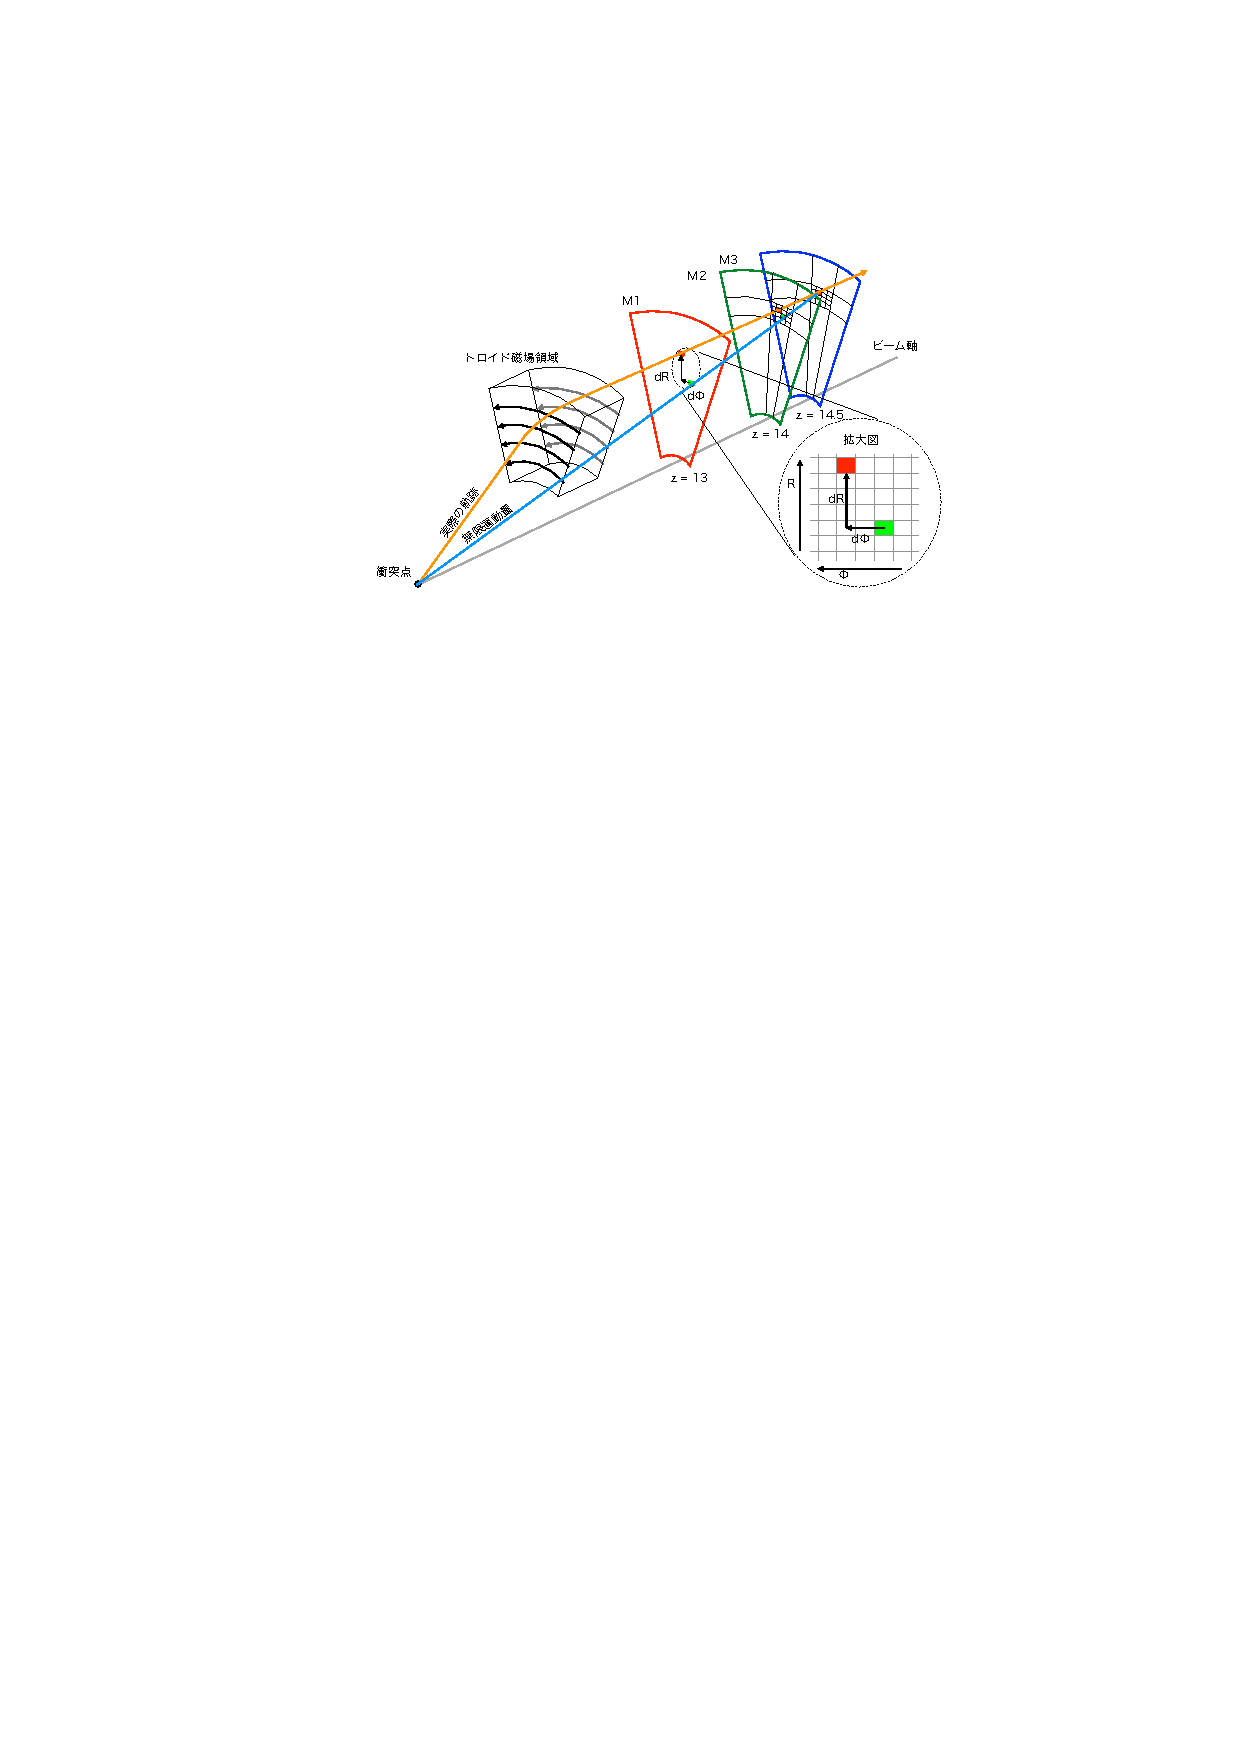
\includegraphics[clip, width=12cm]{fig/3/akatsuka_mt_trigger_scheme.pdf}
  \caption{M3TGCと衝突点を結ぶ直線と実際の飛跡のM1TGCでのずれとdR、d$\phi$の概念図\cite{article:akatsuka}。}
  \label{fig:3-4}
\end{figure}

\begin{figure}[h]
  \centering
  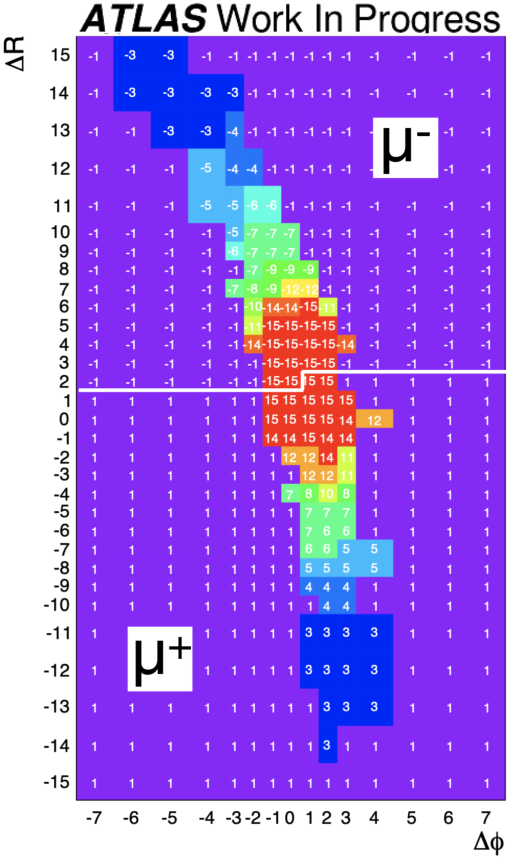
\includegraphics[clip, width=8cm]{fig/3/Run3CW.pdf}
  \caption{Run-3における~Coincidence~Windowの一例\cite{article:shiomi}。}
  \label{fig:3-5}
\end{figure}

%\subsection{後段トリガーシステム~(High Level Trigger)}\label{chapter3-2-2}

\subsection{Level2~Muon~Stand~Alone~(L2MuonSA)}\label{chapter3-2-2}
L2MuonSAはHLTの初段を担っている。
ここではL1から受け取ったRoI周辺のミューオン検出器の情報を用いて、素早くかつL1よりも精密に飛跡を再構成することで高精度の$p_T$を計算し、閾値を設けてトリガー判定を行っている。またL2MuonSAで再構成したミューオンの飛跡候補は、後段のL2MuonCombに送られ、内部飛跡検出器の情報と組み合わせて用いられる。
以下にL2MuonSAの$p_T$再構成の手順を示す。
\begin{enumerate}
    \item RoIの情報をもとに探索範囲であるロードを定義する
    \item ロード内のMDTヒットを用いた各ステーションのスーパーポイント~(SP)の定義
    \item SPから$p_T$に相関のあるパラメータの導出
    \item Look~Up~Table~(LUT)を用いた$p_T$の導出
\end{enumerate}

\subsubsection{ロードの定義}
L2MuonSAではL1から送られてきたRoIの情報をもとに、バレル領域でRPC、エンドキャップ領域ではTGCのヒットを選択し、ミューオンの大まかな飛跡を再構成し、部分飛跡再構成に用いるMDTのヒットの探索領域であるロードを定義する。このロードは、L1におけるロードとは異なるものである。MDTでは$\phi$方向の測定ができないので、RPC、TGCの$\phi$の値をL2MuonSAの$\phi$として用いる。
以下でバレル領域とエンドキャップ領域それぞれでのロードの定義について説明する。

\paragraph{バレル領域におけるロードの定義}
バレル領域では、RoI周辺のRPCのヒットの情報を用いる。
RPCはミドルステーションとアウターステーションに設置されているため、各ステーションでRPCのヒットから大まかな飛跡の位置を求めて、ロードの中心と定義する。インナーステーションにはRPCがないので、ミドルステーションのロード中心を外挿して用いる。

\paragraph{エンドキャップ領域におけるロードの定義}
エンドキャップ領域では、RoI周辺のTGCのヒットの情報を用いる。ミドルステーションでは~TGC~M1、M2、M3、インナーステーションでは~Inner~TGCを用いてロードを定義する。
Inner~TGCがない領域では、ミドルステーションの~TGCの情報を用いて計算した$p_T$と位置情報を用いて飛跡を外挿し、インナーステーションのロードとして定義する。

\subsubsection{SPの定義}
スーパーポイント~(SP)とは、ミューオン検出器でのミューオンの通過位置と通過方向の情報を持った点のことである。
SPは各ステーションにおいて定義したロード内にあるMDTのヒットを直線でフィットして求める。図~\ref{fig:3-6-1}、\ref{fig:3-6-2}にバレル領域におけるロードの求め方を示す。

\begin{figure}[h]
  \begin{minipage}[b]{0.45\linewidth}
      \centering
      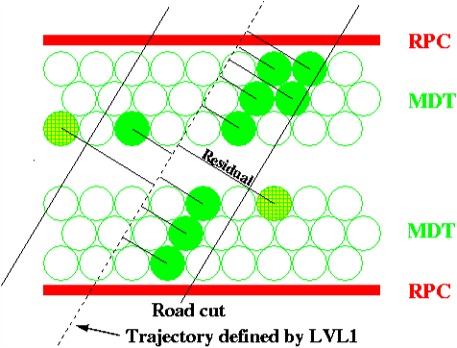
\includegraphics[clip, width=5.5cm]{fig/3/mdtResidual.png}
      \subcaption{各層で1つのMDTヒット選択の例}
      \label{fig:3-6-1}
  \end{minipage}
    \begin{minipage}[b]{0.5\linewidth}
      \centering
      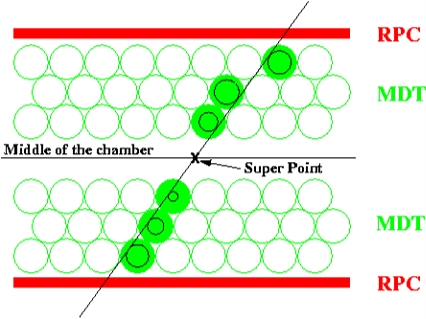
\includegraphics[clip, width=5.5cm]{fig/3/mdtRoad.png}
      \subcaption{ドリフト円のフィッティングからSPの求め方}
      \label{fig:3-6-2}
  \end{minipage}
  \caption{バレル領域におけるロードを用いたSPの求め方\cite{article:onlineMuonReconstruction}。}
\end{figure}

まずRPCのヒットから求めたロードをもとに、MDTのヒットの選別を行う(図~\ref{fig:3-6-2})。ロード内の各MDTヒットに対して、ロード中心からのドリフトチューブの距離~(residual)を計算し、各層について最もロード中心に近いチューブを選択することで各層から最大1つのヒットを用いる。
選択された各ヒットにおいてドリフト時間から距離を計算しドリフト円を定義し、その円のすべてに接する直線を仮定してフィットを行う。
最も$\chi^2$の小さい直線を各ステーションにおけるミューオンの飛跡とし、この飛跡と各ステーションのMDTチェンバーの中心線との交点をSPの$r$、$z$座標とする。また、飛跡の傾きと切片を、SPの傾きと切片と定義する(図~\ref{fig:3-6-2})。

%################################1/20やること!!!!######################################
\subsubsection{SPから$p_T$に相関のあるパラメータの導出}
ミューオンの$p_T$を求めるために、前段階で求めた~SPの傾きの情報を用いて$p_T$と相関のあるパラメータを計算する。

\paragraph{バレル領域における$p_T$と相関のあるパラメータの導出}
バレル領域では、インナー、ミドル、アウターステーションのすべてで磁場領域内に検出器が設置されているので、各ステーションのSPからミューオンの飛跡を再構成し、その曲率半径$R$を$p_T$と相関のあるパラメータとして定義する。
このとき、3つのステーションすべてで~SPを再構成できた場合は3点を用いて曲率半径を計算するが、3つの内2つのステーションのみでしか~SPを再構成できなかった場合は原点からインナーまで$z-R$平面でミューオンが曲がらずに飛んできたことを仮定して曲率半径を計算する。また1つのステーションのみでしか~SPを再構成できなかった場合は、曲率半径を計算できないので$p_T$の再構成を行わない。


\paragraph{エンドキャップ領域における$p_T$と相関のあるパラメータの導出}
エンドキャップ領域では、磁場領域内にインナーと~EE、ミドルステーションが、磁場領域外にアウターステーションが設置されている。
EEチェンバーが設置されている領域~($1.0<|\eta|<1.4$)では、インナーと~EE、ミドルステーションの~SPからミューオンの飛跡を再構成し、バレル領域と同様に曲率半径$R_{curv}$を$p_T$と相関のあるパラメータと定義する(図~\ref{fig:3-7})。
それ以外の領域では磁場領域内にステーションが2つしかなく、SPは最大2つしか再構成されないので曲率半径を計算することは不可能である。なので~L2MuonSAでは磁場に四つ飛跡の曲がりとして角度$\alpha$、$\beta$を定義する。$\alpha$$\beta$は図~\ref{fig:3-8}と~\ref{fig:3-9}で表されるように定義される。
角度$\alpha$は図~\ref{fig:3-8}で表されるように、衝突点とミドルステーションの~SPの位置を結ぶ直線の傾きと、ミドルとアウターステーションの~SPを結ぶ直線の傾きのなす角である。アウターステーションに~SPがない場合はミドルステーションの~SPの傾きを用いる。
角度$\beta$は図~\ref{fig:3-9}で表されるように、インナーステーションでの~SPの傾きとミドル、アウターステーションの~SPを結んだ直線の傾きのなす角である。ここでも角度$\alpha$と同様にアウターステーションに~SPがない場合はミドルステーションの~SPの傾きを用いる。

\begin{figure}[h]
  \centering
  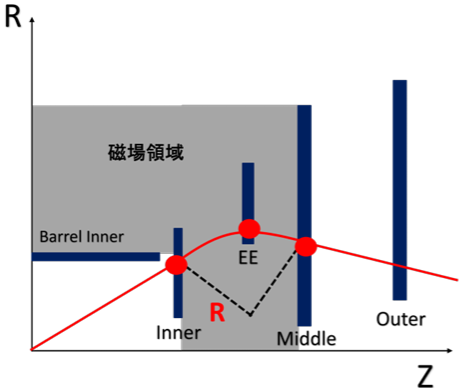
\includegraphics[clip, width=8cm]{fig/3/l2muonSA_Rcurv.png}
  \caption{エンドキャップ領域でのL2MuonSAにおける$R_{curv}$の定義\cite{article:noguchi}。}
  \label{fig:3-7}
\end{figure}

\begin{figure}[h]
  \centering
  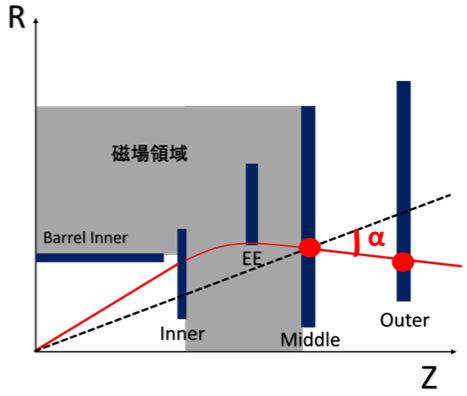
\includegraphics[clip, width=8cm]{fig/3/l2muonSA_alpha.png}
  \caption{エンドキャップ領域でのL2MuonSAにおける$\alpha$の定義\cite{article:noguchi}。}
  \label{fig:3-8}
\end{figure}

\begin{figure}[h]
  \centering
  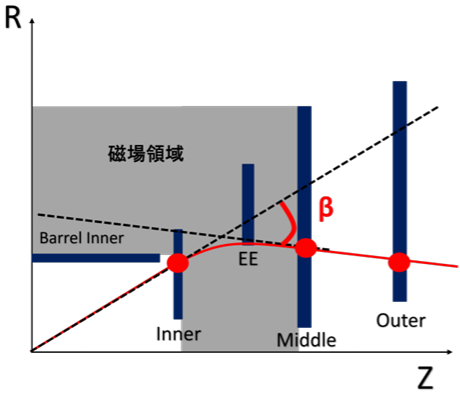
\includegraphics[clip, width=8cm]{fig/3/l2muonSA_beta.png}
  \caption{エンドキャップ領域でのL2MuonSAにおける$\beta$の定義\cite{article:noguchi}。}
  \label{fig:3-9}
\end{figure}



\subsubsection{Look~Up~Table~(LUT)を用いた$p_T$の導出}
全段階で求めた$p_T$と相関のあるパラメータから$p_T$を求める。
このとき高速で処理を行うために、あらかじめ$p_T$と相関のあるパラメータと$p_T$の対応表である~Look~Up~Table~(LUT)をメモリ上に用意しておき、参照することによって即座に$p_T$を導く。
ATLAS検出器では磁場の位置依存性があり、領域によってパラメータと$p_T$の相関は異なるので、セクターや荷電粒子の電荷や、$\eta$、$\phi$などで細かく分割された領域ごとにLUTを作成している。

\paragraph{バレル領域における~LUTを用いた$p_T$の導出手法}
バレル領域では、$\rm{sector}\times Q \times \eta \times \phi = 4\times2\times30\times30$に領域を分割し、それぞれの領域でLUTが作成されている。
sectorは~Large、Small、Large~Special、Small~Specialステーションの4分割、$Q$は荷電粒子の電荷、$\eta$、$\phi$方向はセクターにより異なる範囲で30分割している。
\begin{itemize}
    \item Largeセクター~:~$-1.145<\eta<1.145、-0.230<\phi<0.230$
    \item Smallセクター~:~$-1.050<\eta<1.050、-0.181<\phi<0.181$
    \item Large~Specialセクター~:~$-1.150<\eta<1.150、-0.233<\phi<0.233$
    \item Small~Specialセクター~:~$-1.050<\eta<1.050、-0.181<\phi<0.181$
\end{itemize}


各領域ごとの飛跡の曲率$R_{curv}$と$p_T$の相関は以下の式で表される。
\begin{equation}
    p_T=A \times R_{curv}+B
\end{equation}
この式における$A$、$B$を前もってデータから求めてLUTにまとめることで、飛跡の領域と$R_{curv}$から瞬時に$p_T$を求める。


\paragraph{エンドキャップ領域における~LUTを用いた$p_T$の導出手法}
エンドキャップ領域では、$\eta \times \phi \times (Q \times \eta/|\eta|)= 30\times12\times2$に領域を分割し、それぞれの領域で~LUTが作成されている。$Q$は荷電粒子の電荷で、$\eta/|\eta|$は~A、C-sideを表す。
$\eta$方向はエンドキャップ領域の$1.05<|\eta|<2.50$の範囲で$|\eta|$を30分割、$\phi$方向は$\phi$全体の領域を4回半分に折りたたんでできた領域を12分割している(図~\ref{fig:3-10})。

\begin{figure}[h]
  \centering
  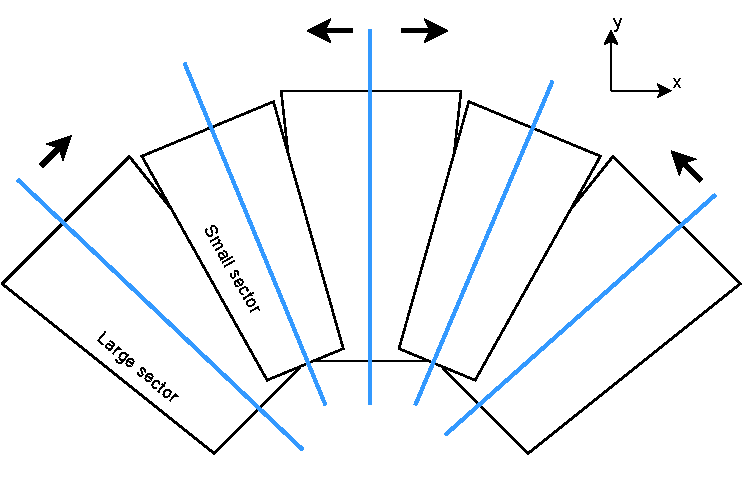
\includegraphics[clip, width=10cm]{fig/3/LUT_binning.pdf}
  \caption{エンドキャップ領域での$\phi$の領域分割の定義。}
  \label{fig:3-10}
\end{figure}

各領域ごとの$\alpha$、$\beta$、$1/R_{curv}$と$p_T$の相関は以下の式で表される。
\begin{equation}
    \alpha, \beta, 1 / R_{\text {curv }}=A \times\left(\frac{1}{p_T}\right)+B \times\left(\frac{1}{p_T}\right)^2
\end{equation}
この式における$A$、$B$を前もってデータから求めてLUTにまとめることで、飛跡の領域と$\alpha$、$\beta$、$1/R_{curv}$から瞬時に$p_T$を求める。$A$、$B$から$p_T$の値への変換は以下の式を用いる。

\begin{equation}
    \frac{1}{p_T}=\frac{-A+\sqrt{A^2+4 B\left(\alpha, \beta, 1 / R_{\text {curv }}\right)}}{2 B}
\end{equation}

$R_{curv}$、$\alpha$、$\beta$それぞれから$p_T$を算出するが、実際にL2MuonSAの$p_T$は1つ選択される。
$R_{curv}$、$\alpha$、$\beta$TGCの情報から計算された$p_T$をそれぞれ$p_{T,R_{curv}}$、$p_{T,\alpha}$、$p_{T,\beta}$、$p_{T,TGC}$と表す。
基本的に磁場内に設置されている検出器3つを用いて求めた$p_{T,R_{curv}}$が最も精度が良い。
そのためEEチェンバーが設置されており、$R_{curv}$が計算できた場合は優先的に$p_{T,R_{curv}}$を使用する。

$p_{T,\alpha}$は衝突点からインナーステーションまでミューオンが曲がらずに飛んでいることを仮定しているが、実際にはカロリメータ等による多重散乱によって飛跡が曲げられることがある。そのためインナーチェンバーを使用する$p_{T,\beta}$の方が分解能が良い。
しかし$\beta$はミドルステーションとアウターステーションに加えてインナーステーションのSPの情報を用いるので、インナーでSPの再構成を間違える割合の分だけ$p_T$の再構成を間違える割合が増える。インナーはミューオン絵¥検出器の最内層なので、カロリメータから漏れ出てくるミューオン以外の荷電粒子の数が多いため、$p_T$の計算を間違える場合が多い。そのため、$p_{T,\alpha}$と$p_{T,\beta}$は使い分ける必要があるので、$R_{curv}$による$p_T$の計算に失敗した場合は図~\ref{fig:3-11}を用いて$p_T$の選択を行う。

\begin{figure}[h]
  \centering
  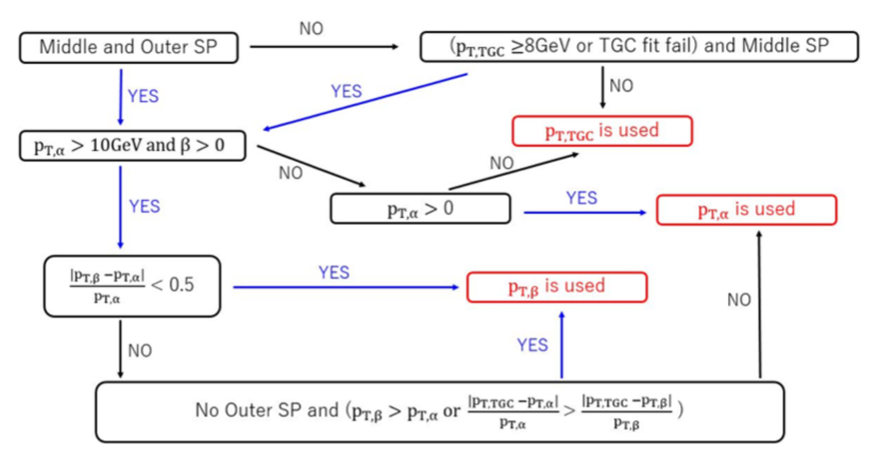
\includegraphics[clip, width=14cm]{fig/3/l2muonSA_pTselection.png}
  \caption{エンドキャップ領域でのL2MuonSAにおける$p_{T,R_{curv}}$、$p_{T,\alpha}$、$p_{T,\beta}$、$p_{T,TGC}$の選択条件\cite{article:wakamiya}。}
  \label{fig:3-11}
\end{figure}


\subsection{Level2~Combined~Muon~(L2MuComb)}\label{chapter3-2-3}
Level-2~Combined~Muon~(L2MuComb)では、L2MuonSAで計算した飛跡と内部飛跡検出器の情報を組み合わせてミューオンの$p_T$の再構成を行い、トリガー判定を行う。
まず、L2MuonSAで再構成した飛跡を内部飛跡検出器の位置まで外挿する。外挿された飛跡の周辺で、内部飛跡検出器で測定されたミューオン候補の飛跡を探索する。見つかった飛跡とL2MuonSAの飛跡の$\chi^2$を$\eta$、$\phi$、$p_T$などの情報を用いて計算し、最も$\chi^2$の小さい飛跡の$p_T^{ID}$を取得する。
この$p_T^{ID}$とL2MuonSAの$p_T^{SA}$で、分解能に基づく重み~($w^{SA}$、$w^{ID}$)を用いて加重平均を取ることでL2MuCombにおける$p_T^{CB}$を計算する。

\begin{equation}
    \frac{1}{p_T^{C B}}=\frac{w^{S A} \cdot \frac{1}{p_T^{S A}}+w^{I D} \cdot \frac{1}{p_T^{I D}}}{w^{S A}+w^{I D}}
\end{equation}

\subsection{Event~Filter~(EF)}\label{chapter3-2-4}
Event Filter~(EF)では、全検出器の情報を用いてミューオンの飛跡を再構成する。
再構成アルゴリズムはオフライン再構成アルゴリズムとほとんど同じものを用いるので、精密な飛跡の再構成を行うことが可能である。
基本的には$p_T$に対して閾値を設定することでミューオンの選別を行うが、ミューオンの内部飛跡検出器での飛跡の周辺に他のミューオンが存在しないこと~(アイソレーション)を要求した選別も可能である。このような$p_T$以外の要求による選別は、$p_T$の閾値を低くした場合のバックグラウンドを削減でき、トリガーレートを抑制できるため、低い$p_T$のミューオンを含む事象を取得するために有用である。

\section{第3期運転~(Run-3)における新ミューオントリガーアルゴリズム}\label{chapter3-3}
2014年から2022年までのロングシャットダウンを経て、2023年から第3期運転が開始された。Run-3から新たに様々なトリガーが導入されたが、本論文では近接2ミューオンのためのトリガーとRun-3から新たに導入された検出器であるNSWを用いたミューオントリガーについて取り上げる。

\subsection{近接2ミューオンのためのトリガーアルゴリズム}\label{chapter3-3-1}

\subsection{NSWを用いたL2MuonSAでの部分飛跡再構成アルゴリズム}\label{chapter3-3-2}
第2章で述べたように、NSWはRun-3からLHCのルミノシティ増加に伴い検出器のヒットレートが増加することに対応するために導入された検出器である。
Run-3で運用が始まる前に、L2MuonSAでNSWを用いて部分飛跡を再構成するアルゴリズムが開発されシミュレーションでの性能評価を経て導入された。


\subsection{本論文の目的}\label{chapter3-4}